              
                %%%%%%%%%%%%%%%%%%%%%%%%%%%%%%%%%%%%%%%%%%%%%%%%%%%%%%%%%%%%%%%%%%%%%%
% LaTeX Example: Project Report
%
% Source: http://www.howtotex.com
%
% Feel free to distribute this example, but please keep the referral
% to howtotex.com
% Date: March 2011 
% 
%%%%%%%%%%%%%%%%%%%%%%%%%%%%%%%%%%%%%%%%%%%%%%%%%%%%%%%%%%%%%%%%%%%%%%
% How to use writeLaTeX: 
%
% You edit the source code here on the left, and the preview on the
% right shows you the result within a few seconds.
%
% Bookmark this page and share the URL with your co-authors. They can
% edit at the same time!
%
% You can upload figures, bibliographies, custom classes and
% styles using the files menu.
%
% If you're new to LaTeX, the wikibook is a great place to start:
% http://en.wikibooks.org/wiki/LaTeX
%
%%%%%%%%%%%%%%%%%%%%%%%%%%%%%%%%%%%%%%%%%%%%%%%%%%%%%%%%%%%%%%%%%%%%%%
% Edit the title below to update the display in My Documents
%\title{Project Report}
%
%%% Preamble
\documentclass[paper=letter, fontsize=11pt]{scrartcl}
\usepackage{url}
\usepackage{color}
\usepackage{fourier}
\usepackage{listings}
\usepackage[T1]{fontenc}
\usepackage[spanish]{babel}
\selectlanguage{spanish}
\usepackage{hyperref}
\usepackage[pdftex]{graphicx}
\usepackage[margin=2.5cm]{geometry}
\usepackage{amsmath,amsfonts,amsthm} % Math packages
                                       % English language/hyphenation
\usepackage[protrusion=true,expansion=true]{microtype}  

%%% Maketitle metadata
\newcommand{\horrule}[1]{\rule{\linewidth}{#1}}     % Horizontal rule

\title{
        %\vspace{-1in}  
        \usefont{OT1}{bch}{b}{n}
        \normalfont \normalsize \textsc{Universidad de los Andes, Departamento de F\'isica \\
        F\'isica at\'omica} \\ [25pt]
        \horrule{0.5pt} \\[0.4cm]
        \huge Helio excitado \\
        \horrule{2pt} \\[0.5cm]
}
\author{
        \normalfont                                 \normalsize
        Juan Barbosa, 201325901\\[-3pt]      \normalsize
        Abril 18, 2017
}
\date{}

\lstset{keywordstyle=\color{blue}, basicstyle=\tiny, frame=single, language=Python}

%%% Begin document
\begin{document}
\maketitle

\[
\boxed{-\dfrac{\hbar^2}{2m}\nabla^2\Psi(x) + V(x)\Psi(x) = E\Psi(x)}
\]

Para el \'atomo de helio la ecuaci\'on anterior se escribe usando coordenedas esf\'ericas, el m\'etodo de Hartree consiste en relajar el potencial que actua sobre un electr\'on. Dado que ambos electrones comparten tres n\'umeros cu\'anticos y que la ecuaci\'on de Schr\"odinger no incluye el sp\'in, se consideran indistinguibles. El m\'etodo consiste en considerar un \'unico electr\'on a la vez, junto con el potencial producido por los otros dos. Usando consideraciones geom\'etricas, en las cuales a distancias grandes el electr\'on observar\'a el potencial de una carga puntual con carga $Z-1$ para distancias cortas el efecto ser\'a an\'alogo a un monopolo. 
\begin{equation}
	\begin{matrix}
		V(r) = -\dfrac{Zke^2}{r} \qquad r \ll 1 \\
		V(r) = -\dfrac{ke^2}{r} \qquad r \gg 1
	\end{matrix}
\end{equation}

Haciendo un cambio de variable $r=\dfrac{a_0}{z}u$ y la energ\'ia propia del sistema:
\begin{equation}
	\begin{matrix}
		\dfrac{V(u)}{E_0} = -\dfrac{2}{u} \qquad u \ll 1 \\
		\dfrac{V(u)}{E_0} = -\dfrac{2}{Zu} \qquad u \gg 1
	\end{matrix}
\end{equation}

Este potencial se usa \'unicamente para la primera iteraci\'on, por lo cual no es del todo relevante cual es la forma exacta del mismo para puntos interm\'edios, dado que con cada iteraci\'on el sistema es relajado hasta la estabilidad.
\begin{equation}
	\dfrac{V(u)}{E_0} = -\dfrac{2}{Zu}\left(1+(Z-1)e^{-u}\right)
\end{equation}

Usando la probabilidad radial $P=4\pi R^2r^2/\int Pdr$ se determina la densidad de carga del electr\'on.
\begin{equation}
	\dfrac{Q}{e}(u) = -(Z-1)\int\limits_{0}^{u}P(w)dw
\end{equation}


El potencial se obtiene integrando sobre el campo
\begin{equation}\label{eq: V1}
	V_{1}(u) = -\left(V_0 + \dfrac{Z}{u} +  \int\limits_{0}^{u}\dfrac{2}{Z}\dfrac{Q/e}{u^2}\right)
\end{equation}
donde $V_0$ se ajusta de tal forma que el potencial converja para distancias grandes y $Z/u$ corresponde con el potencial del n\'ucleo.

La implementaci\'on se realiza en C, y una \'ultima parte en Python para graficar. Se usan 10000 puntos entre $U=0$ y $U=30$. La ecuaci\'on diferencial a resolver es:
\begin{equation}
	\dfrac{d^2R}{du^2} + \dfrac{2}{u}\dfrac{dR}{du} + \left(\epsilon -V_{1}(u) - \dfrac{l(l+1)}{u^2}\right)R = 0
\end{equation}

Lo anterior para el electr\'on en el nivel $1s$, para el segundo electr\'on se realiza un proceso an\'alogo donde $V_1$
ser\'a el potencial que sentir\'a el electr\'on 2. Teniendo el potencial para $V_2$ se calcula el potencial producto a su presencia de manera an\'aloga a \autoref{eq: V1} donde se encuentra $V_2 + V_N$. Este potencial se usa nuevamente para calcular la funci\'on de onda para el electr\'on en el estado $1s$. El proceso se realiza 50 veces.

\lstinputlisting[language=C]{atom.c}
\lstinputlisting[]{plotter.py}

\begin{figure}[!ht]
	\centering
	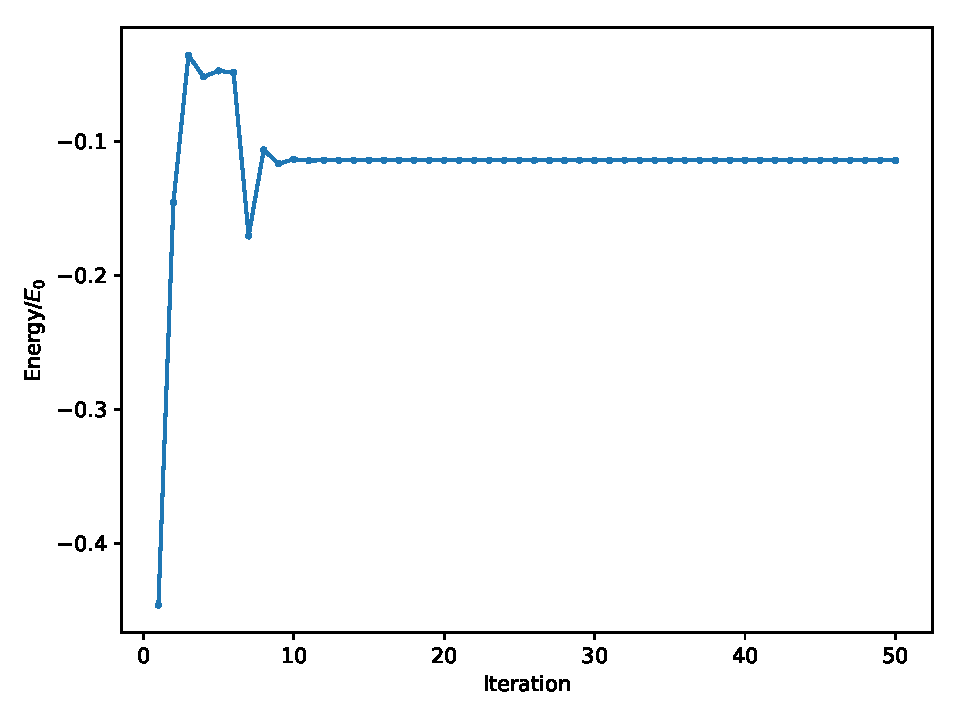
\includegraphics[width=0.6\linewidth]{change.pdf}
	\caption{Evoluci\'on de la energ\'ia $\epsilon_2$ con 50 iteraciones.}
	\label{fig:prop}
\end{figure}

La \autoref{fig:prop} muestra el comportamiento del potencial en para las distintas iteraciones. Las energ\'ias se muestran en la parte inferior, de donde se observa que se estabilizan para $\epsilon_2=-0.114$:

La funci\'on radial resultante para cada electr\'on se muestra en la siguiente figura. Adem\'as se grafican la probabilidad radial, la densidad de carga y el comportamiento del potencial a distancias cortas y largas.
\begin{figure}[!h]
	\centering
	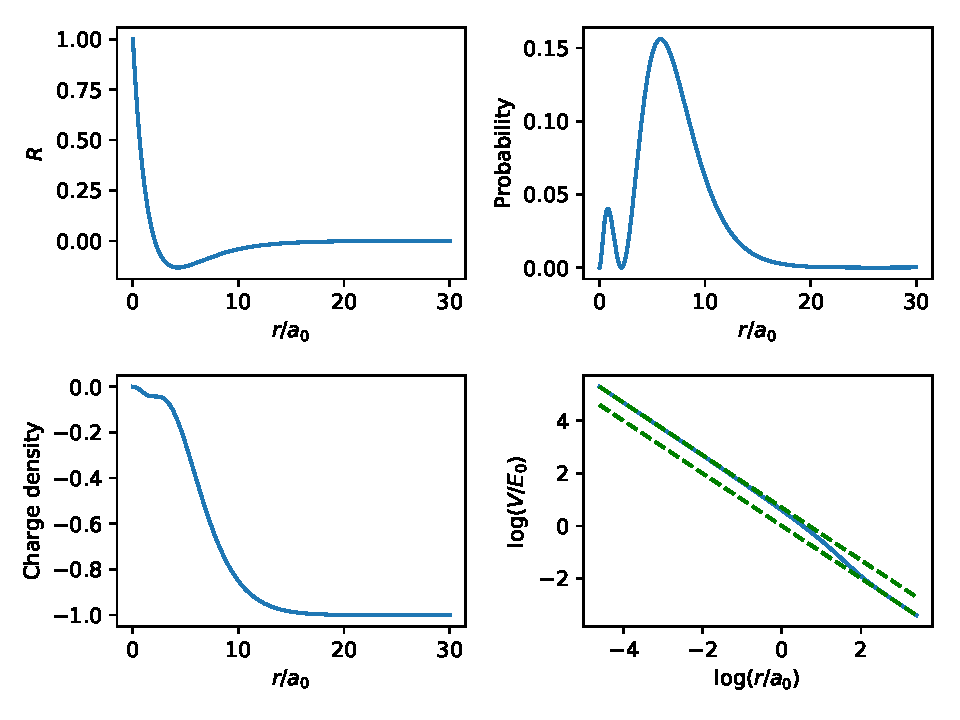
\includegraphics[width=0.7\linewidth]{complete.pdf}
	\caption{Distintas propiedades de la funci\'on encontrada luego de 50 iteraciones.}
\end{figure}

La disminuci\'on en la energ\'ia se debe a que ya no existe la misma repulsi\'on electr\'onica debido a que la distancia entre los electrones es mayor producto de encontrarse en dos niveles de energ\'ia distintos.
\end{document}
              